\chapter{异域脉冲(Exotic pulses)}
\label{ch:Exotic}

对于一根光纤来说,如果$\gamma\neq 0$和$\betag_2\neq 0$,发射到光纤中的脉冲会以多种令人惊讶的方式演变。从本质上讲,非线性会根据脉冲的功率曲线改变脉冲的局部频率,而色散则会导致不同频率相对于载波频率前进或延迟,这反过来又会改变功率曲线。本章将探讨这两种效应在不同的 $\gamma$ 和 $\betag_2$ 值下的相互作用。

\section{基本孤子}
\label{sec:soliton}
考虑一下 $\gamma>0$ 的光纤。如图 ~\ref{fig:chirp_profiles}所示,这将导致脉冲前缘(后缘)产生红(蓝)色偏移。正如在 Sec.~\ref{sec:GVD} 中解释的那样,$\betag_2<0$ 意味着蓝光比红光传播得更快,从而导致脉冲的前缘(后缘)变得更蓝(更红)。如果根据瞬时功率曲线,$\gamma>0$ 会使脉冲的前缘(后缘)更红(蓝),而根据场的二次导数,$\betag_2<0$ 会使脉冲的前缘(后缘)更蓝(红),那么我们自然会问,是否存在一个脉冲包络,在这个脉冲包络中,这两种效应在每个瞬间都完全平衡,因此脉冲的形状在向前传播时不会改变。对于这样的脉冲,场包络应该与距离无关,而相位应该与时间无关,即

\begin{align}
    \A(z,T) &= V(T)e^{i\phi(z)}
\end{align}
解方程 
\begin{align}
\label{eq:NLSE_soliton}
    \partial_z\A &=  -i  \frac{\betag_2}{2}\partial_T^2\A+i\gamma|\A|^2\A.
\end{align}
正如\href{https://github.com/OleKrarup123/NLSE-vector-solver/blob/main/TutorialVideos/Soliton-Video/Fundamental_soliton_derivation.pdf}{此节}推导所解释的那样,可以证明解是
\begin{align}
    \A(z,T) &= \sqrt{\frac{|\betag_2|}{\gamma T_0^2}}\cdot\text{sech}\left(\frac{T}{T_0}\right)\exp\left(i\frac{|\betag_2|}{2T_0^2}z\right),
\end{align}
其中,$T_0$ 是脉冲场下降到其峰值的 64.8\% 时的时间。这种以双曲正割包络为特征的稳定脉冲被称为 “基本孤子”。高斯脉冲与双曲正割脉冲的对比见图 ~\ref{fig:gauss_sech}。请注意,双曲正割脉冲的峰值功率($\A_{max}$)必须选择为正好等于特征振幅($\A_{char}=\sqrt{|\|betag_2|/\gamma T_0^2}$),这样才能实现稳定传播!
\begin{figure}
    \centering
    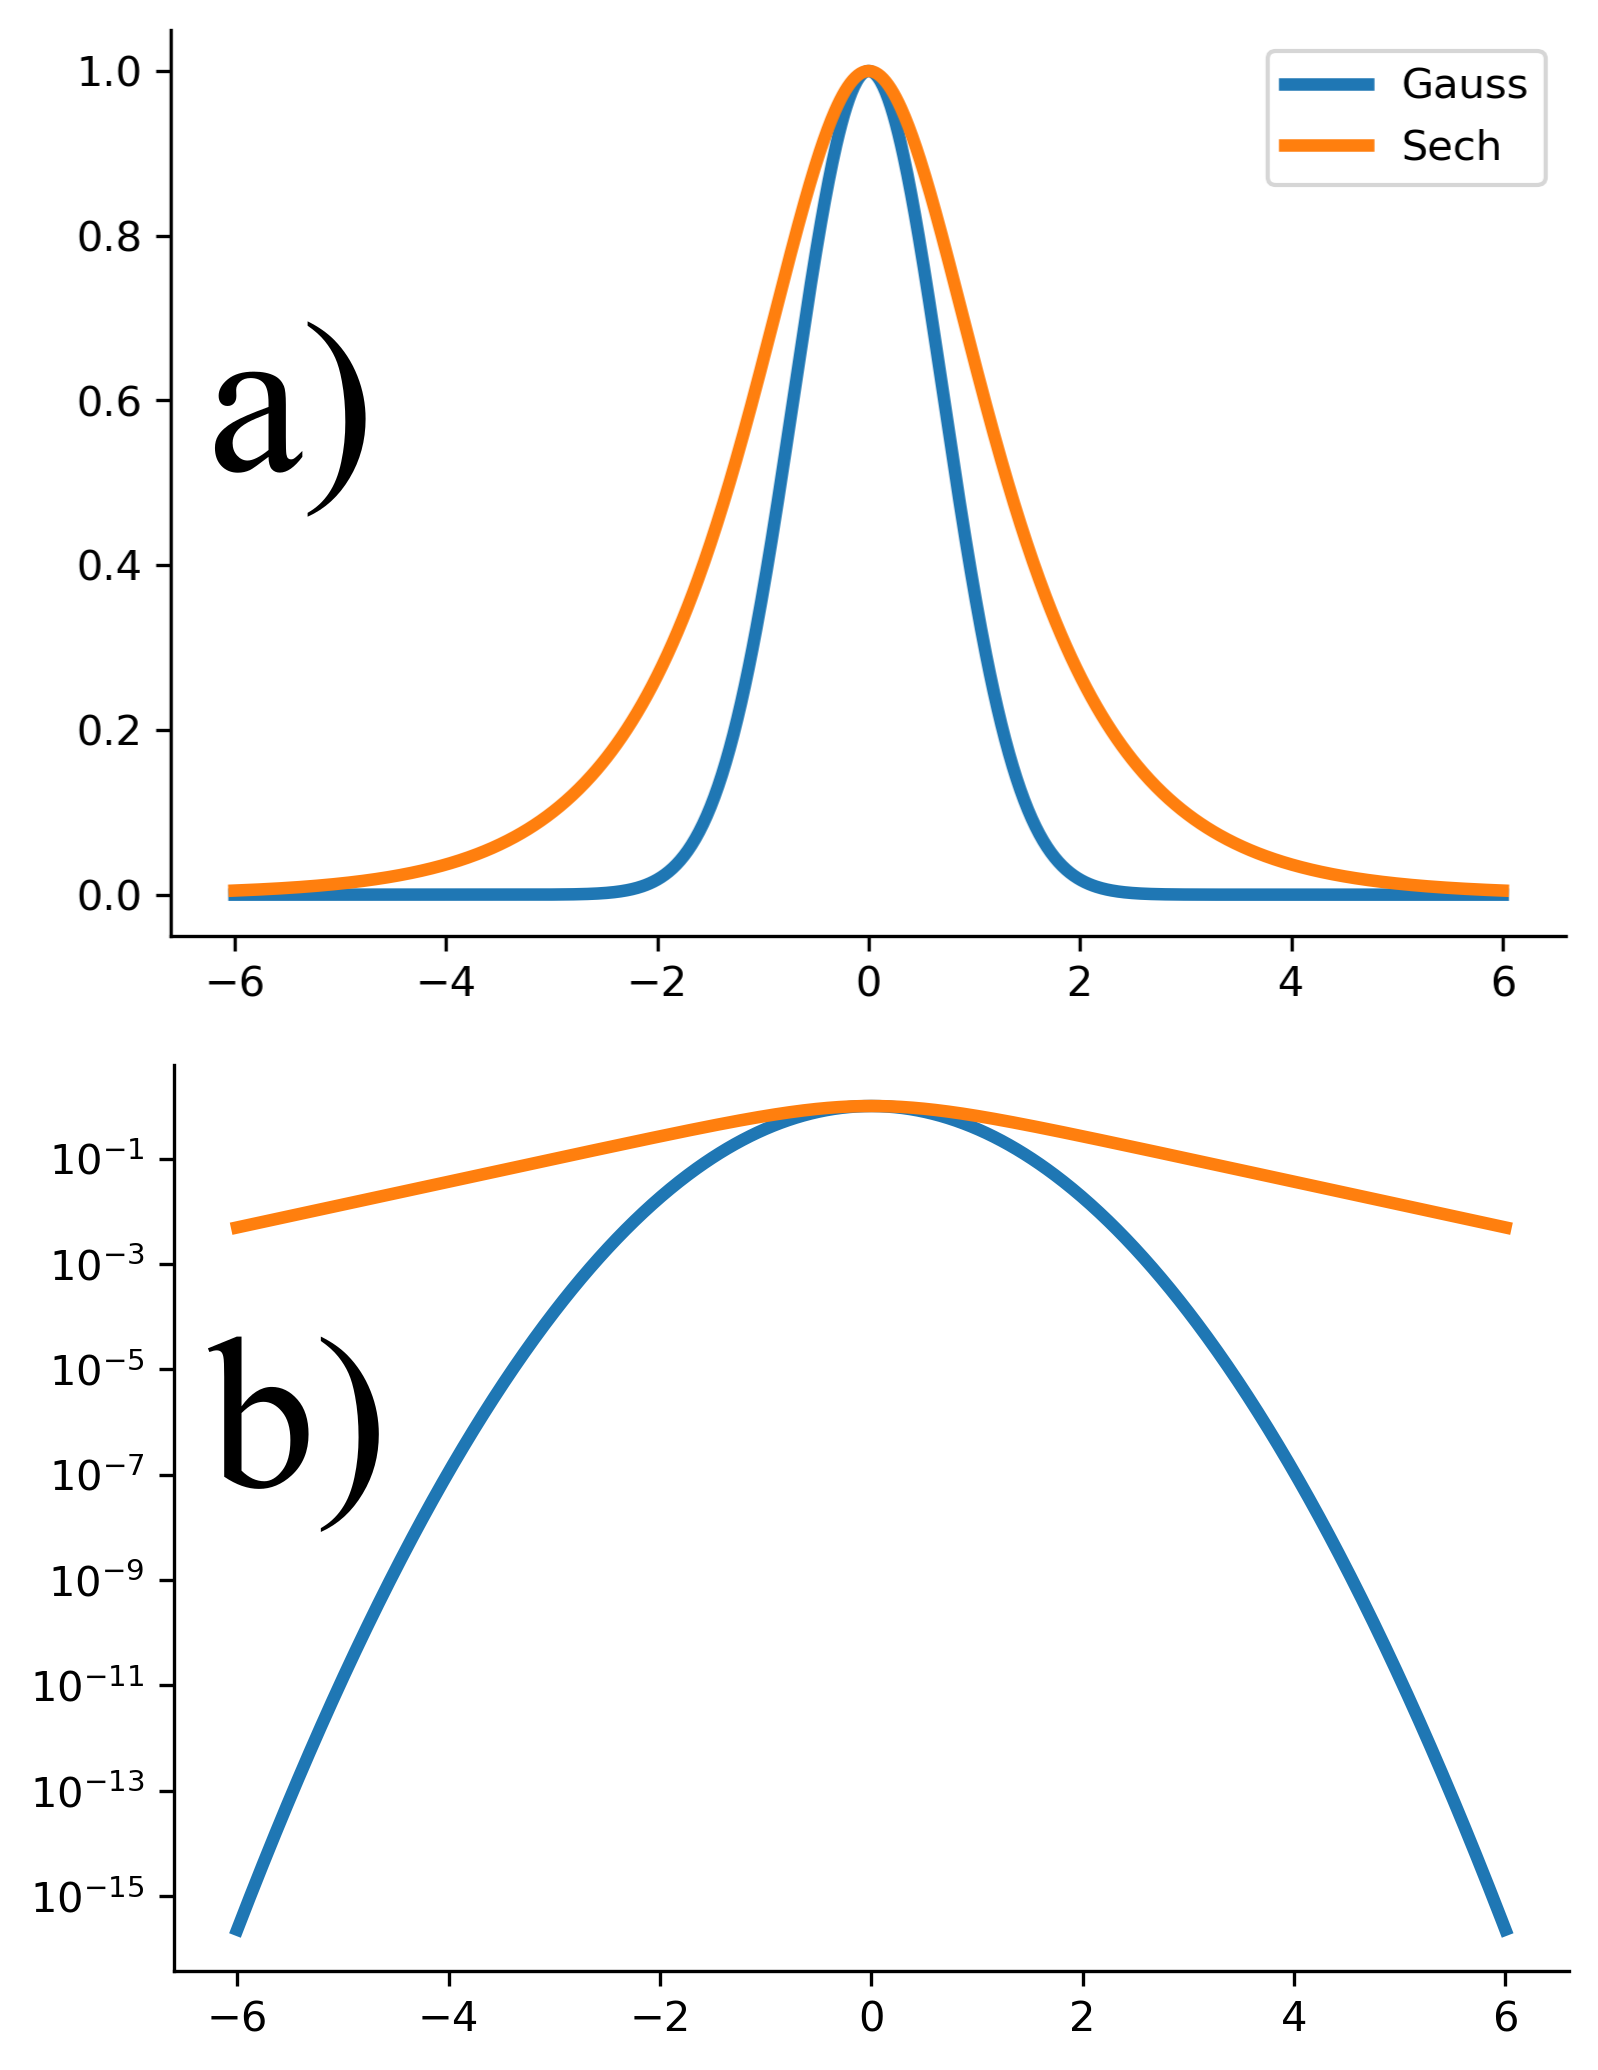
\includegraphics[width=1\linewidth]{figures/gauss_sech_comparison.png}
    \caption{高斯脉冲与双曲正割脉冲的比较,a) 为线性比例,b) 为对数比例。  }
    \label{fig:gauss_sech}
\end{figure}
\subsection{通信中的孤子}
在接近193~THz($\approx$1550~nm)的近红外频率的硅光纤中,由于$\gamma>0$和$\betag_2<0$,基底孤子曾一度在电信领域引起极大兴趣,因为它们的抗色散能力和恒定形状可以减少符号间干扰。然而,在小节{subsec:ZDF}中提到的电子色散补偿方面的改进同样使孤子在光纤通信中的应用过时了。取而代之的是采用所谓“\href{https://www.youtube.com/watch?v=hCk_cg-OfUQ}{root-raised-cosine}”场包络的脉冲。  

\section{Higher order Solitons}
如果双曲正割脉冲的峰值功率小于 $P_{char}=|\A_{char}|^2=|\betag_2|/\gamma T_0^2$,那么与色散相比,非线性效应将过于微弱,无法形成基本孤子。因此,当脉冲向前传播时,它在时域中的范围会扩大。如果峰值功率增大到超过 $P_{char}$,脉冲在演化过程中就会出现 “振荡”。在 $\A_{max}$ 是 $\A_{char}$ 整数倍的特殊情况下,振荡孤子的演化会特别乖巧。关于 $\A_{max}=3\A_{char}$ 的孤子的时间和频谱演化示例,请参见 Fig.~\ref{fig:Soliton_comparison}~a-b)。有关光纤中孤子的更多信息,请参见 \href{https://youtu.be/KAZ7pCQ-x8Y}{本视频教程}。
\subsection{孤子分裂}
\label{subsec:fission}

基阶孤子和高阶孤子可以看作是公式 ~\ref{eq:NLSE_soliton} 的 “固定点(fixed point)”。然而,公式~\ref{eq:NLSE_soliton}本身只是公式~\ref{eq:GNLSE}的近似,而公式~\ref{eq:GNLSE}对影响光脉冲在色散和非线性介质中传播的物理学原理提供了更一般的描述。事实证明,除了 $\gamma>0$ 和 $\betag_2<0$ 之外,其他效应的存在最终会扰乱初始孤子脉冲的演化。在图 ~\ref{fig:Soliton_comparison}~c-d)中,$\betag_3>0$ 的存在会导致一个高阶孤子在传播 0.5 米的距离后,由于 FWM 而 “裂变 ”成两个较弱的新频率孤子。其他效应,如自膨胀效应、拉曼效应,甚至与理想的孤子脉冲一起传播的光噪声所引起的调制不稳定性,也同样会导致孤子裂变。因此,就像一支铅笔在笔尖上保持平衡一样,孤子传播应被视为一种不稳定的平衡。有关孤子裂变的更多详情,请参阅 \href{https://youtu.be/tHpIR2Kuxp0}{本视频教程}。
\begin{figure}
    \centering
    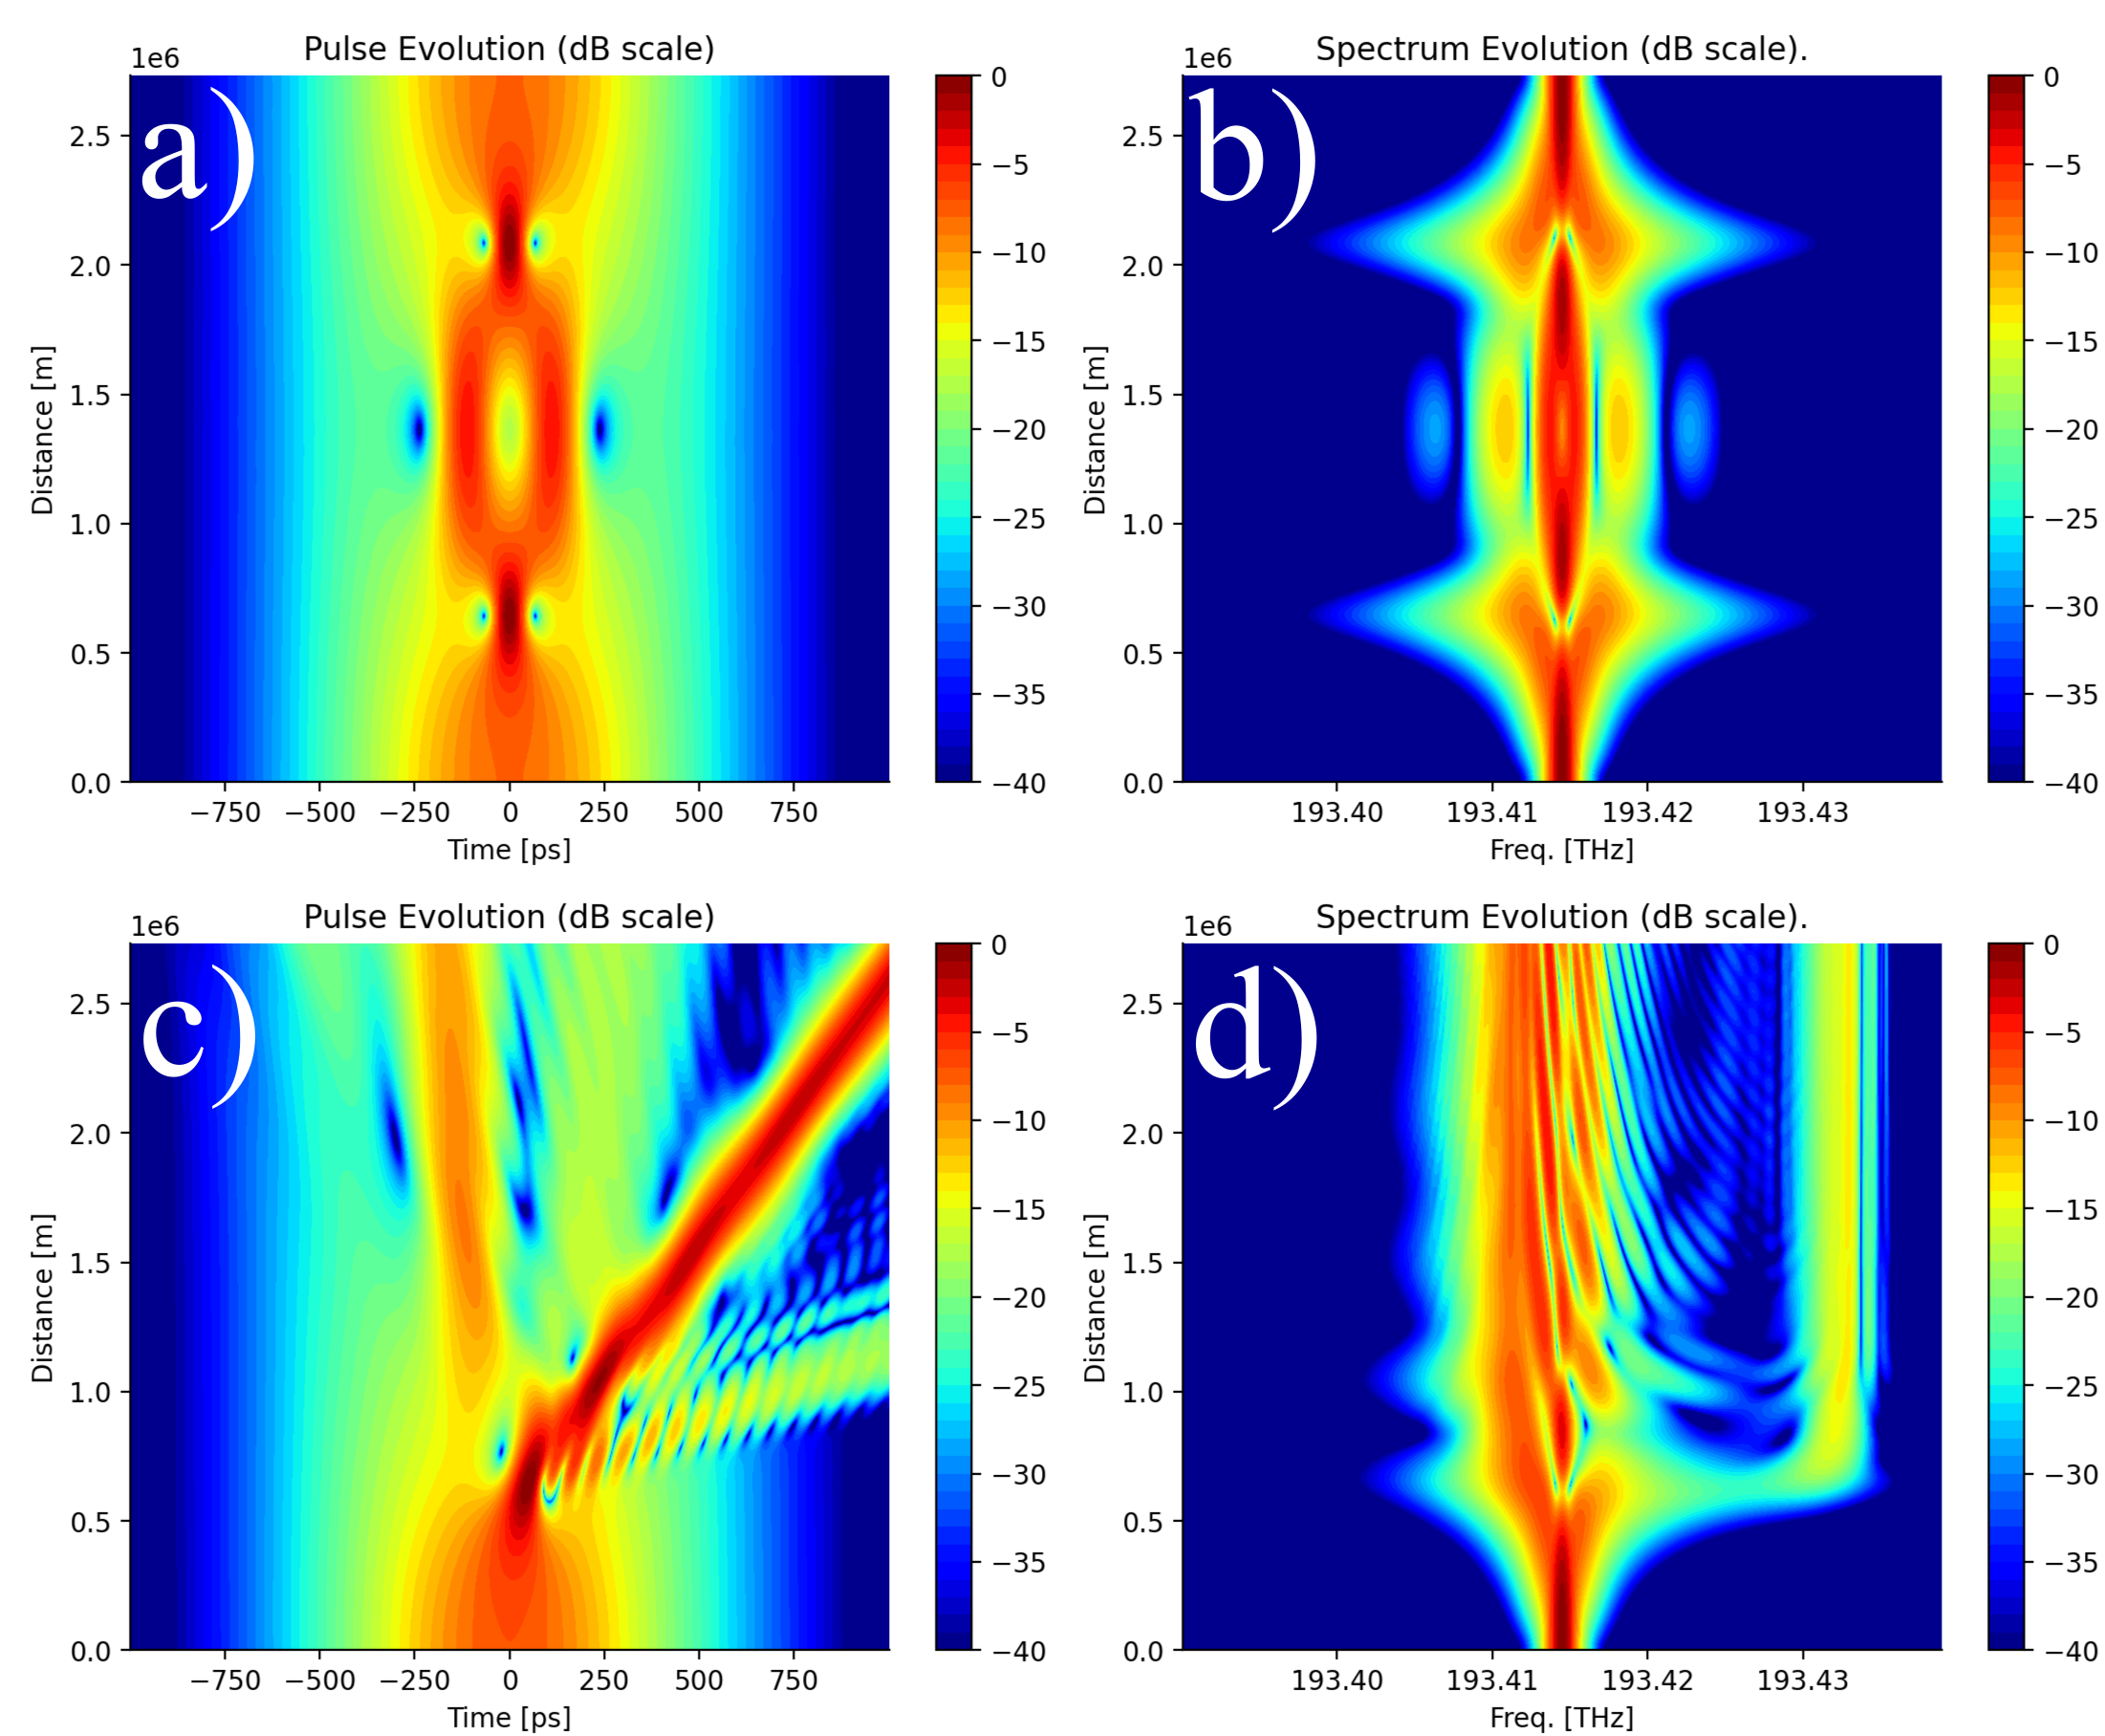
\includegraphics[width=1\linewidth]{figures/Soliton_comparison.png}
    \caption{a) $N=3$ 孤子的时间演变,其中 $\A_{max}=3\A_{char}=3\sqrt{|\betag_2|/\gamma T_0^2}$。b) $N=3$ 孤子的频谱演化。) 与 a-b) 中相同的 $N=3$ 孤子的时间和光谱演变,但光纤的 $\betag_3>0$ 导致脉冲 “裂变”,从而说明了孤子传播的不稳定性。这些图是利用 \href{https://colab.research.google.com/drive/123pT-IsLWIEZY9XW3-1WzkTXfg1IEkkD?usp=sharing}{本互动笔记本}中的数值模拟生成的,我们鼓励读者进行实验。}
    \label{fig:Soliton_comparison}
\end{figure}





\section{光学波破裂(Optical Wave Breaking)}
当海浪接近海滩时,水开始在波浪的前缘“堆积”,最终导致波浪在冲击海岸之前“破裂”。在非线性光纤中,当 $\gamma>0$ 且 $\betag_2>0$ 时,也可以观察到类似的现象。与第~\ref{sec:soliton}节中讨论的当 $\betag_2$ 为负时非线性和色散的平衡不同,现在它们是“协同作用”的。非线性使脉冲的前缘(后缘)变得更红(更蓝),而色散使红色(蓝色)光的传播速度比载波快(慢)。结果是任何脉冲都会在时间域迅速展宽。通常,这种展宽方式会使脉冲的前后功率逐渐“堆积”,从而导致功率斜率变陡,进而生成更大的频率调制(chirp),由于色散的影响,导致脉冲的时间展宽更加快速。当斜率变得足够陡峭时,色散会像水波崩溃一样,将新产生的频率从主脉冲中“推出”。图~\ref{fig:OWB_and_similariton}~a-b)说明了这一现象,称为“光学波破裂”(OWB)。尽管OWB对入射脉冲的变化可能是有害的,但如果想要一个具有陡峭斜率且峰值功率大致恒定的光学脉冲,它也可以是有益的。有关OWB的更多细节,请参阅\href{https://youtu.be/XEx6lOf6f40}{此视频教程}。

\subsection{相似孤子(Similaritons)}
当 $\gamma>0$ 且 $\betag_2>0$ 时,OWB使脉冲在时间域扩展,从而减小其峰值功率。如果进一步假设 $\alpha>0$,意味着脉冲在传播过程中会被放大,那么这种峰值功率的损失会不断被补偿。实际上,在这种情况下,任何输入脉冲(无论其初始形状如何)都会演化为一个具有抛物形功率包络的脉冲,如图~\ref{fig:OWB_and_similariton}~c)所示,并且脉冲的调制将呈现线性变化,从前到后依次变为红色和蓝色~\cite{Similariton_evolution}。这种“相似孤子”的峰值功率和持续时间会随着传播距离的增加而不断增加,具体解释请参见\href{https://youtu.be/ZtWIRaj5VV4}{此视频教程}。相似孤子可以出现在某些光学放大器中,并且由于其线性变化的频率调制,它们是通过诺贝尔奖获得的方法——啁啾脉冲压缩——生成具有极高峰值功率脉冲的理想候选者,详细内容可见\href{https://youtu.be/Eh5CHRWFT-M}{此视频教程}。

\begin{figure}
    \centering
    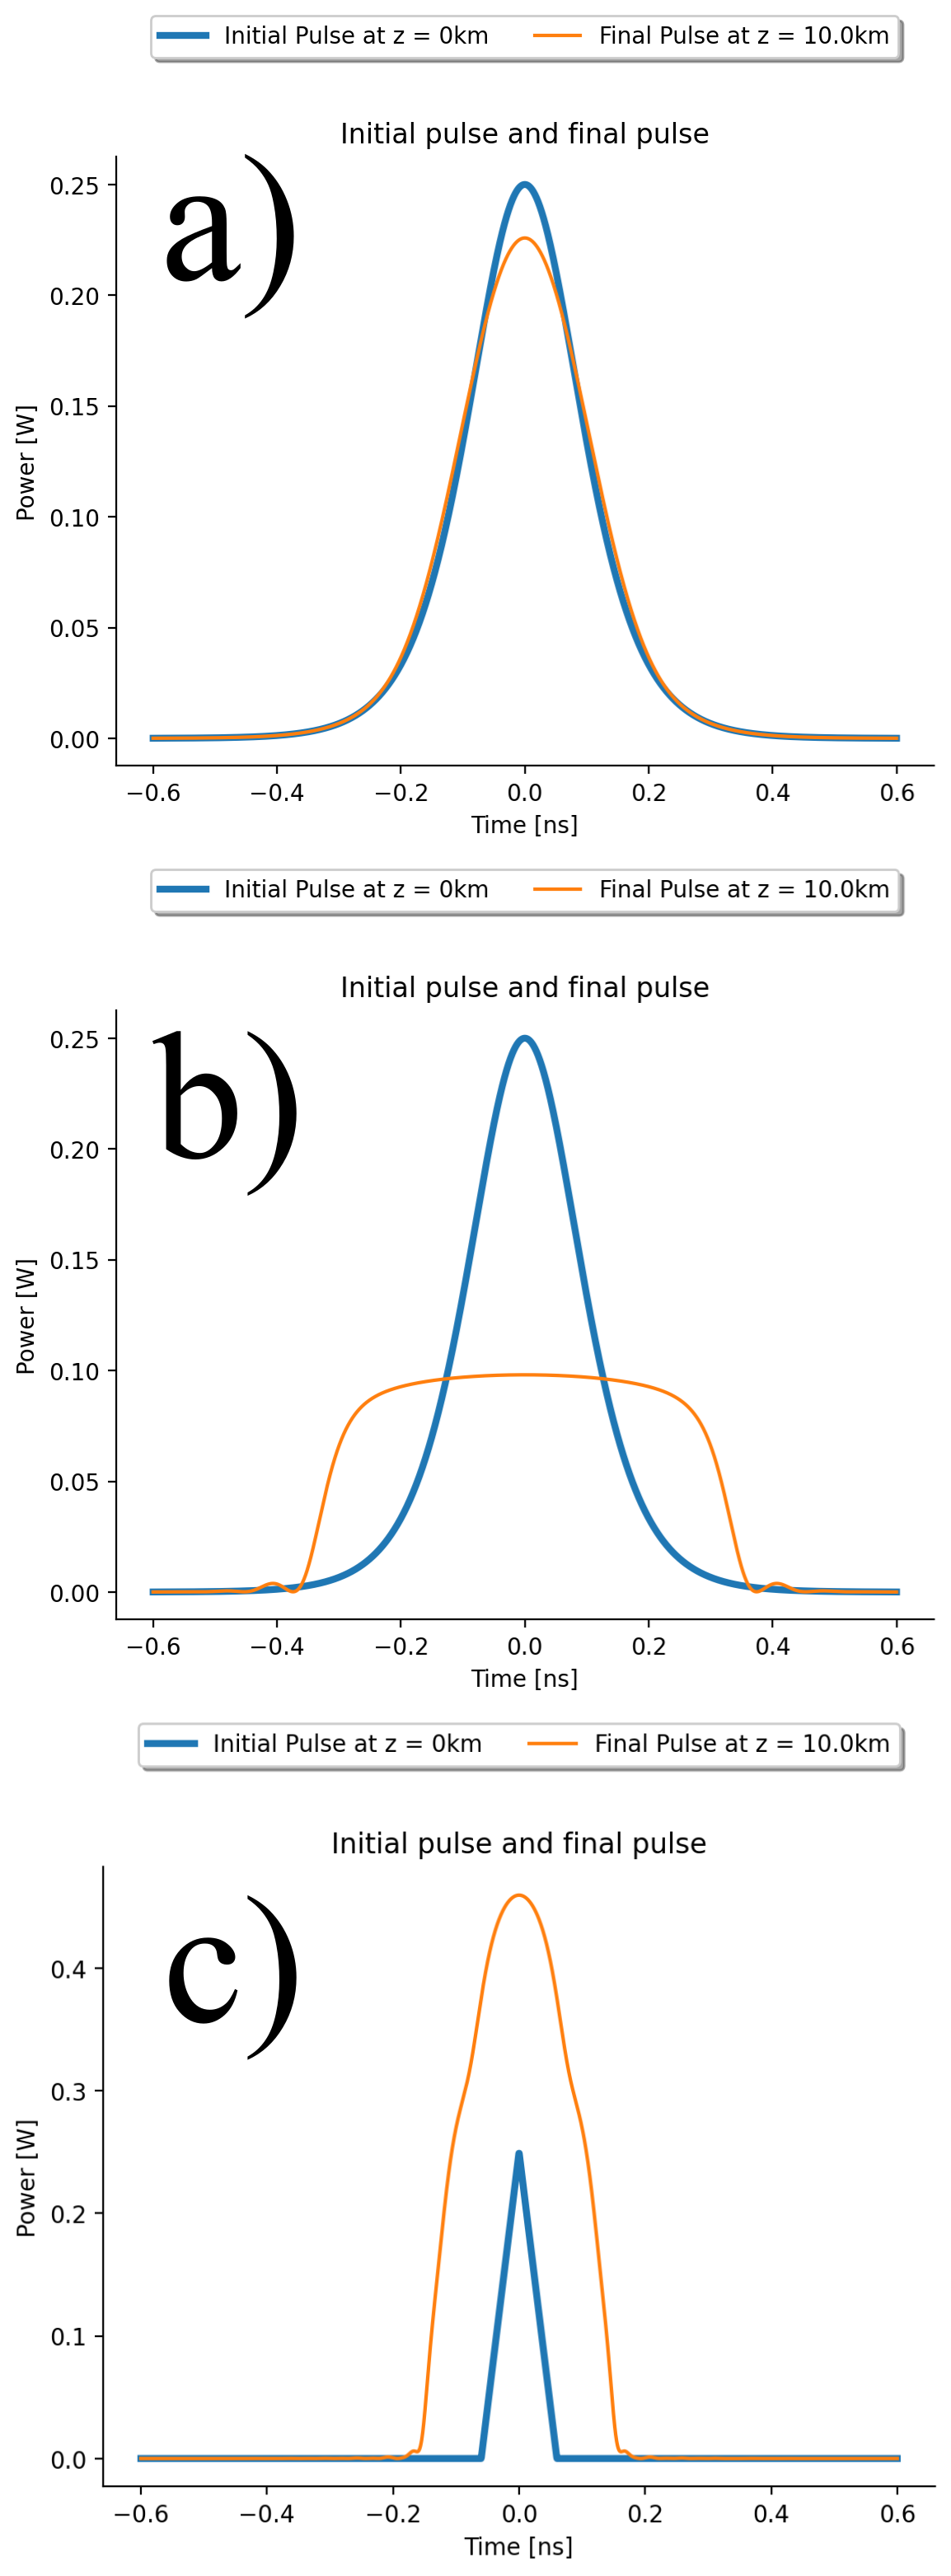
\includegraphics[width=0.5\linewidth]{figures/OWB_and_similariton.png}
    \caption{a)双曲正割脉冲在介质中的演变,其中$\betag_2>0$。b)与a)中相同的脉冲在介质中的演变,其中$\betag_2>0$和$\gamma>0$导致功率在脉冲前后 “堆积”,从而导致OWB。这些图是使用 \href{https://colab.research.google.com/drive/1qtMcXElXn4VBntfCgXIGGkyDfiGicElx?usp=sharing}{本互动笔记本}中的数值模拟生成的,我们鼓励读者进行实验。}
    \label{fig:OWB_and_similariton}
\end{figure}

\section{新型孤子}

\subsection{暗孤子(Dark Solitons)}
通常,光脉冲由突然增加的激光功率组成,前后则是长时间零功率。肉眼看到的脉冲就像是在黑暗的房间里,灯被短暂地打开一样。只要满足第~\ref{sec:soliton}节中描述的条件,这样的脉冲可以稳定地通过非线性介质传播。我们可以考虑在非线性介质中,所谓的“反脉冲”——一个高功率的连续波(CW)信号,经历一个短暂的功率下降,类似于灯短暂熄灭后再被重新点亮。它将由功率下降的前沿和功率上升的后沿组成。如果 $\gamma>0$ 且 $\betag_2>0$,前沿(后沿)会变得更蓝(更红),使得这部分光传播速度变慢(加速)。类似于第~\ref{sec:soliton}节的情况,可以计算出非线性和色散恰好平衡的场包络是一个双曲正切函数,从而形成一个稳定传播的“暗孤子”,其表达式为:

\begin{align}
    \A(z,T) = \A_{char}\tanh\left(\frac{T}{T_0}\right)\exp\left(i\frac{|\betag_2|}{T_0^2}z \right).
\end{align}

有关暗孤子的更多信息,请参见\href{https://youtu.be/MrNfI1_eTZ0}{此视频教程}。

\subsection{拉曼孤子(Raman Solitons)}
如果拉曼效应存在,并且脉冲谱向较低频率移动,那么在 $\betag_2<0$ 的非线性介质中可以形成一个“拉曼孤子”。这个孤子保持其包络的形状,但会经历一个恒定的红移,并由于 $\betag_2<0$ 使得红光比蓝光传播得更慢,进而产生越来越大的时间延迟,如图~\ref{fig:dark_and_raman}c-d)所示。拉曼孤子通常出现在脉冲的孤子裂变之后,这些脉冲的持续时间通常在几十飞秒的量级。有关拉曼孤子的解释,请参见\href{https://www.youtube.com/watch?v=K33YUfegL1w}{此视频教程}。

\begin{figure}
    \centering
    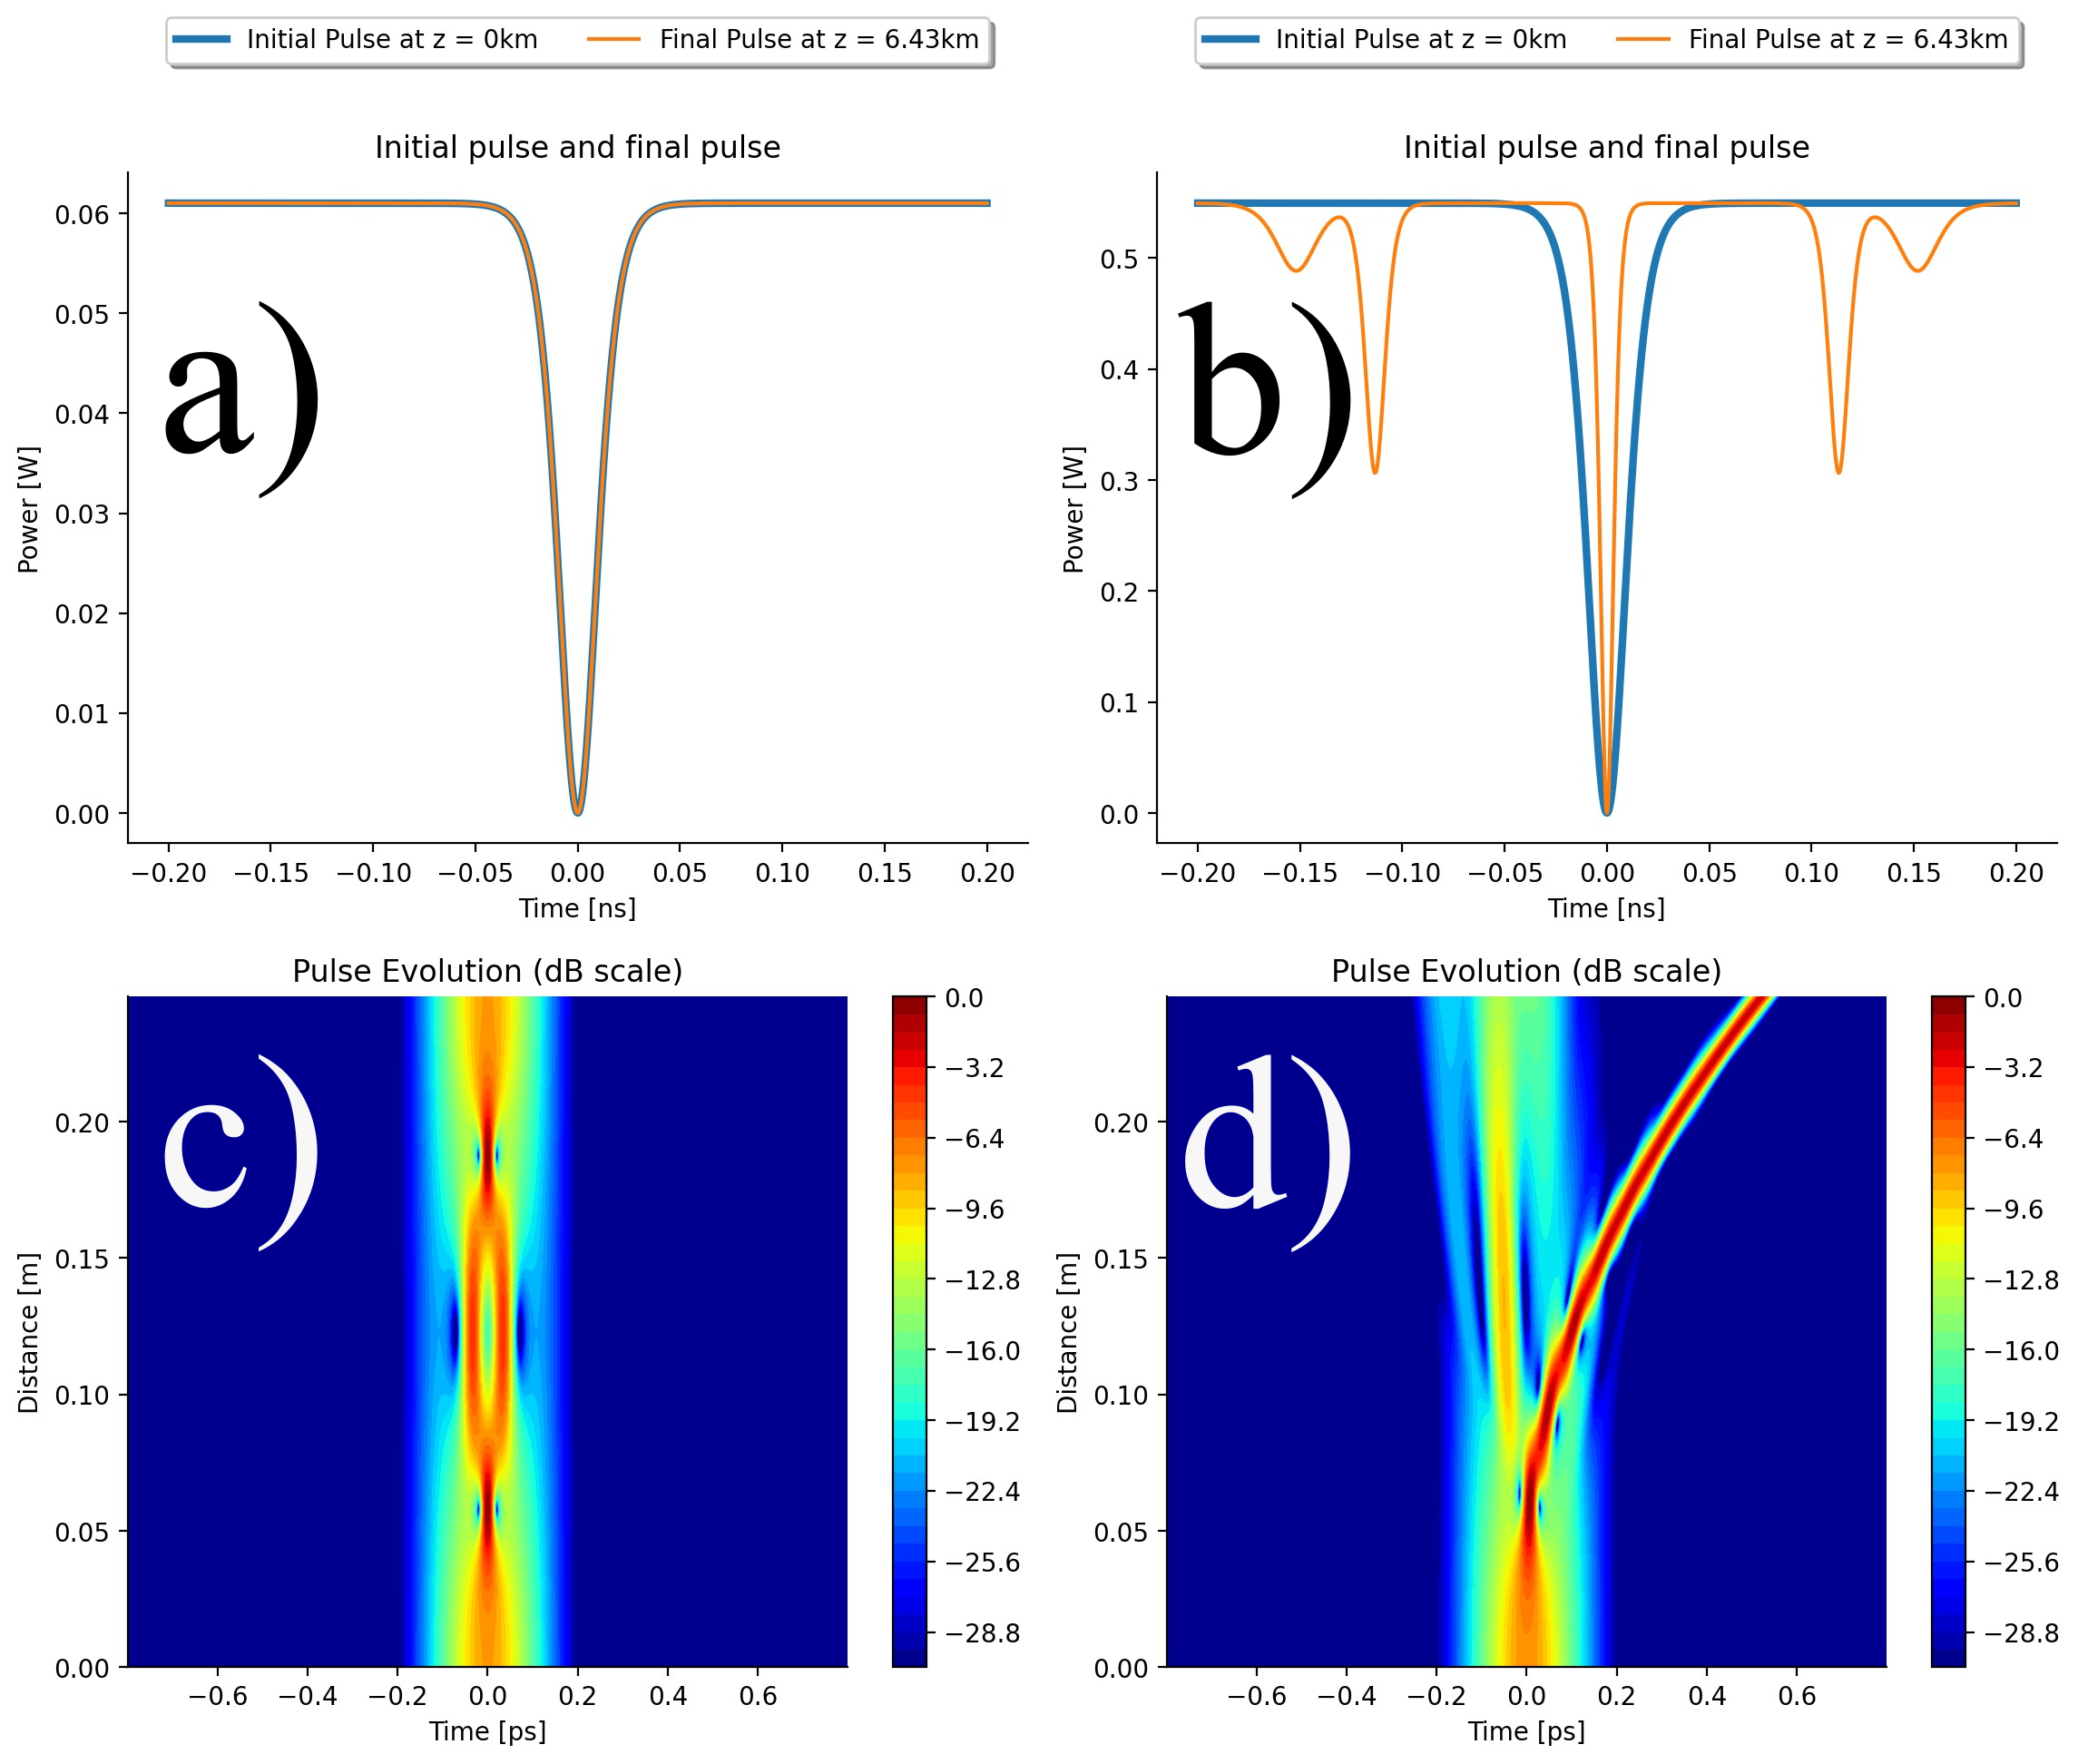
\includegraphics[width=1\linewidth]{figures/dark_and_raman_soliton_combined.png}
    \caption{a) 基本暗孤子在介质中稳定传播,其中 $\betag_2>0$ 和 $\gamma>0$. b) 一个 N=3 的暗孤子在介质中传播,与 a 中相同。c) 一个 N=3 的孤子在$\betag_2<0$和$\gamma>0$的介质中传播。 d) 与 c) 中相同的脉冲在相同的介质中传播,除了公式 ~\ref{eq:raman_basic} 所描述的拉曼效应被考虑在内,导致孤子裂变并产生一个自漂移拉曼孤子。这些图是使用 \href{https://colab.research.google.com/drive/1qtMcXElXn4VBntfCgXIGGkyDfiGicElx?usp=sharing}{这个互动笔记本}生成的,我们鼓励读者进行实验。}
    \label{fig:dark_and_raman}
\end{figure}

\subsection{矢量孤子(Vector Solitons)}
在第~\ref{Sec:XPM}节中,已经展示了不同频率的光可以通过非线性效应相互影响相位。同样,在非线性介质中,两种不同的光偏振也可以相互影响相位。通过使用方程~\ref{eq:GNLSE} 的矢量版本,其中 $\gamma>0$,$\betag_2<0$,且介质中光沿 x 和 y 轴的折射率不同,可以得到所谓的“矢量孤子”的解析表达式。对于这些情况,孤子的特殊情况是圆偏振光和偏振方向为 $45^{o}$ 的线性偏振光~\cite{AGRAWAL_CH6_POL}。






